\chapter{Resultate}
\label{resultate}
Wie schon an verschiedenen Stellen in dieser Diplomarbeit erw�hnt, sind mit den vorgestellten Verfahren Partikelsimulationen mit minimalem Speicherbedarf m�glich. Laut Windows Taskmanager ben�tigt die Simulation, aus der die folgenden Screenshots stammen, bei 830 dargestellten und 4000 f�r die Physik verwendeten Partikeln f�r die Physik und die Oberfl�chenberechnung gemeinsam unter 20MB. Dabei h�ngt der Speicherbedarf linear von der Partikelanzahl, der Anzahl der Oberfl�chenpunkte und der Anzahl der Zellen, die Fl�ssigkeit enthalten, ab.

Die Bildwiederholfrequenz liegt bei dieser Simulation auf einem Athlon 1.2GHz PC mit ATI Radeon 9600 zwischen 16 und 70 Bildern pro Sekunde.

Die Bilder in diesem Kapitel sind meist Stereoskopien, also Bilder der selben Szene aus leicht variierten Blickwinkeln.
Betrachtet man diese Bilder, indem man versucht, hindurch zu blicken, so erfasst das linke Auge das linke Bild und das rechte Auge das rechte Bild und es entsteht ein dreidimensionaler Eindruck. Um das Fokussieren zu erleichtern, ist eine m�glichst helle Beleuchtung hilfreich.

Auf diese Weise kann schon bei der Punktewolke in Bild \ref{fig:ss7fit} die r�umliche Verteilung dieser Punkte erfasst werden. Diese Punkte sind die Zentren der Partikel, auf denen die Physik simuliert wird.
\begin{figure}[htb]
	\begin{center}
	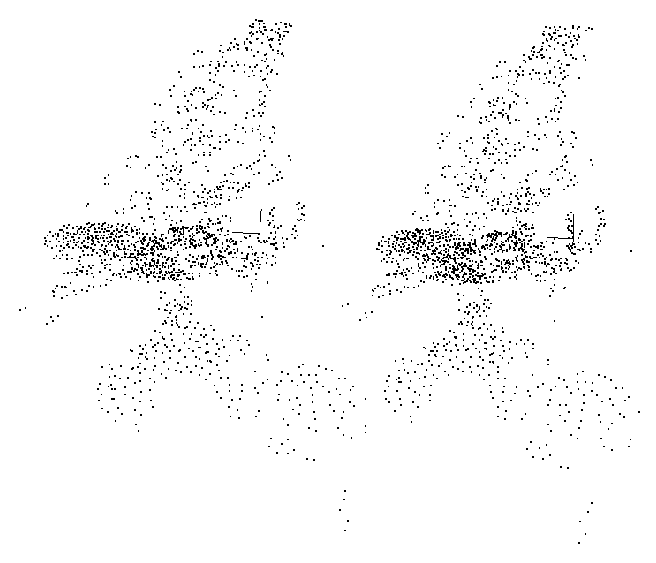
\includegraphics{pix/ss7fit.eps}
	\caption{Partikel einer Fl�ssigkeit, die auf eine Ebene str�mt.}
	\label{fig:ss7fit}
	\end{center}
\end{figure}

In Bild \ref{fig:ss6} wird die selbe Punktverteilung, allerdings mit den Verfahren aus Kapitel \ref{vis}, dargestellt. Die Oberfl�che ist rund und wirkt organisch.
\begin{figure}[htb]
	\begin{center}
	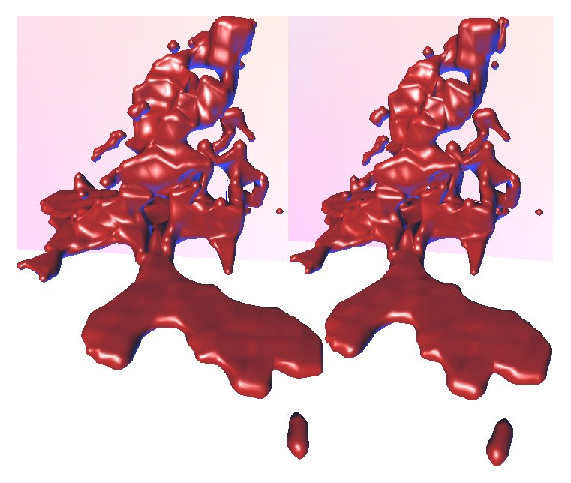
\includegraphics{pix/ss6.eps}
	\caption{Die Oberfl�chendarstellung zur Partikelverteilung aus Abb. \ref{fig:ss7fit}.}
	\label{fig:ss6}
	\end{center}
\end{figure}

Ohne Abrunden der Oberfl�che sieht man allerdings sofort, dass das Gitter des Marching Cube Algorithmus sehr grob ist (siehe Abb. \ref{fig:3d4}). Tropfen erscheinen als Oktaeder, die Lichtquellen erzeugen keine Spiegellinien.
\begin{figure}[htb]
	\begin{center}
	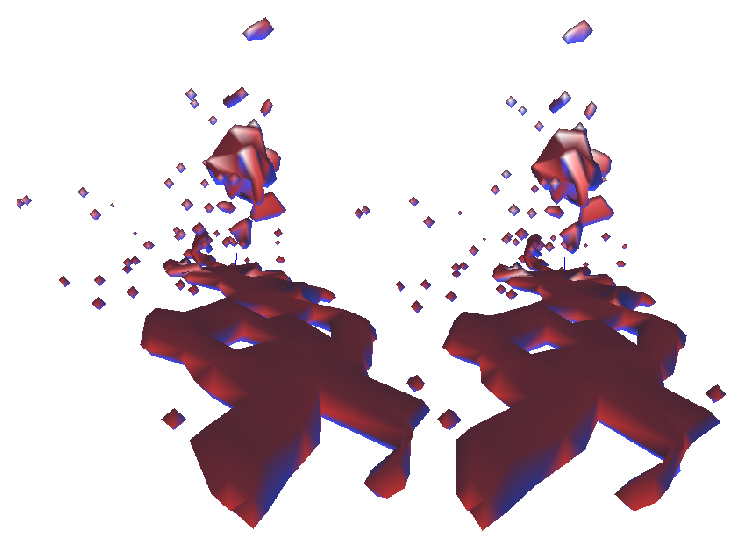
\includegraphics{pix/3d4.eps}
	\caption{Ohne ATI-TRUFORM wirkt alles eckig und man sieht keine Spiegellinien.}
	\label{fig:3d4}
	\end{center}
\end{figure}

Dass die wie in Abb. \ref{fig:ueberschneid} (a) auf Seite \pageref{fig:ueberschneid} dargestellte �berschneidung von Fl�chen auch tats�chlich beobachtet werden kann, zeigt Bild \ref{fig:ss8}. Entartungen, wie in Bild \ref{fig:entartet} (a) beschrieben, sind mir seit der Verfeinerung des Gitters nicht mehr aufgefallen.
\begin{figure}[htb]
	\begin{center}
	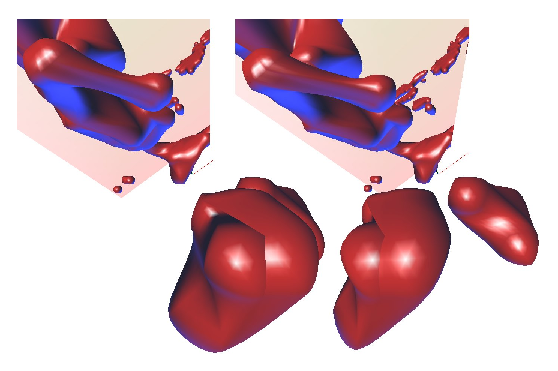
\includegraphics{pix/ss8.eps}
	\caption{Selbst�berschneidung der Oberfl�che.}
	\label{fig:ss8}
	\end{center}
\end{figure}

In Abb. \ref{fig:spritzwasser} verteilen sich Partikel auf einem gro�en Gebiet. Gerade in Szenen, in denen nicht viele Partikel interagieren, ist die Bildrate besonders hoch. Auch wenn hier ca. 5.000\footnote{5.000 mal 64 wegen der ATI-TRUFORMs.} Dreiecke die Oberfl�che darstellen, werden noch �ber 35 Bilder pro Sekunde erreicht. Die Oberfl�chenberechnung wird nur dann langsam, wenn sich viel Oberfl�che auf der selben $z$-Koordinate befindet.
\begin{figure}[htb]
	\begin{center}
	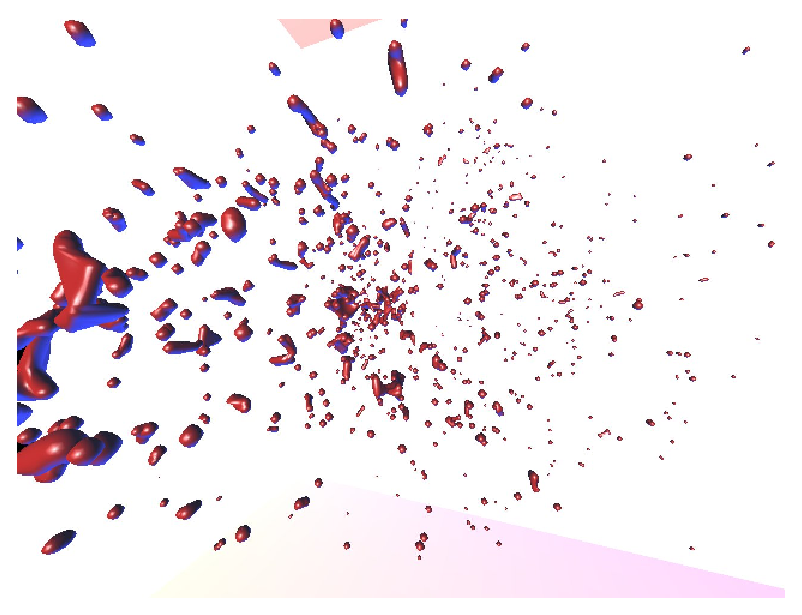
\includegraphics{pix/spritzwasser.eps}
	\caption{Spritzeffekt.}
	\label{fig:spritzwasser}
	\end{center}
\end{figure}
\chapter{Ausblick}
\label{ausblick}
Auch wenn die hier gezeigten Resultate noch nicht nach Wasser aussehen, denke ich, dass schon bald erste Anwendungen entwickelt werden, die vielleicht nur kleine Mengen Wasser, oder zumindest nicht-transparente Fl�ssigkeiten, in interaktiven Umgebungen integriert zeigen werden.

Obwohl das Trennen und Vereinen von Tropfen mit meinem Marching-Cube-Algorithmus unsch�ne Artefakte erzeugt, kann er eventuell in modifizierter Form, insbesondere mit einem besseren Algorithmus zur Bestimmung der Normalen als schnelle Methode zur Erzeugung runder H�llfl�chen weiter Anwendung finden.

Ver�nderungen, die n�tig w�ren, um Fl�ssigkeiten verschiedener physikalischer Eigenschaften zu simulieren stehen in keinem Widerspruch zu den vorgestellten Methoden. Im Gegenteil. So wie die Kontrollpartikel nur in der Physik von den Fl�ssigkeitspartikeln unterschieden werden, k�nnten auch, theoretisch beliebig viele, verschiedene Fl�ssigkeiten miteinander interagieren.

\chapter{Danksagung}

Abschlie�end m�chte ich mich bei den Mitarbeitern des Lehrstuhls f�r Computer Graphik \& Visualisierung der TU M�nchen, insbesondere Herr Prof. Dr. Westermann, sowie bei Prof. Dr. Huckle bedanken, dass sie meine Diplomarbeit in dieser Form m�glich gemacht haben. Aber auch Freunde und Familie die mir mit Rat und Tat zur Seite standen m�chte ich danken.